
\documentclass[border=10pt, 12pt]{standalone}
\usepackage[svgnames]{xcolor}
\usepackage{amsmath}
\usepackage{pgfplots}
\pgfplotsset{compat=newest}
\usepackage[sfdefault]{FiraSans}
\usepackage{FiraMono}
\renewcommand*\familydefault{\sfdefault}
\begin{document}
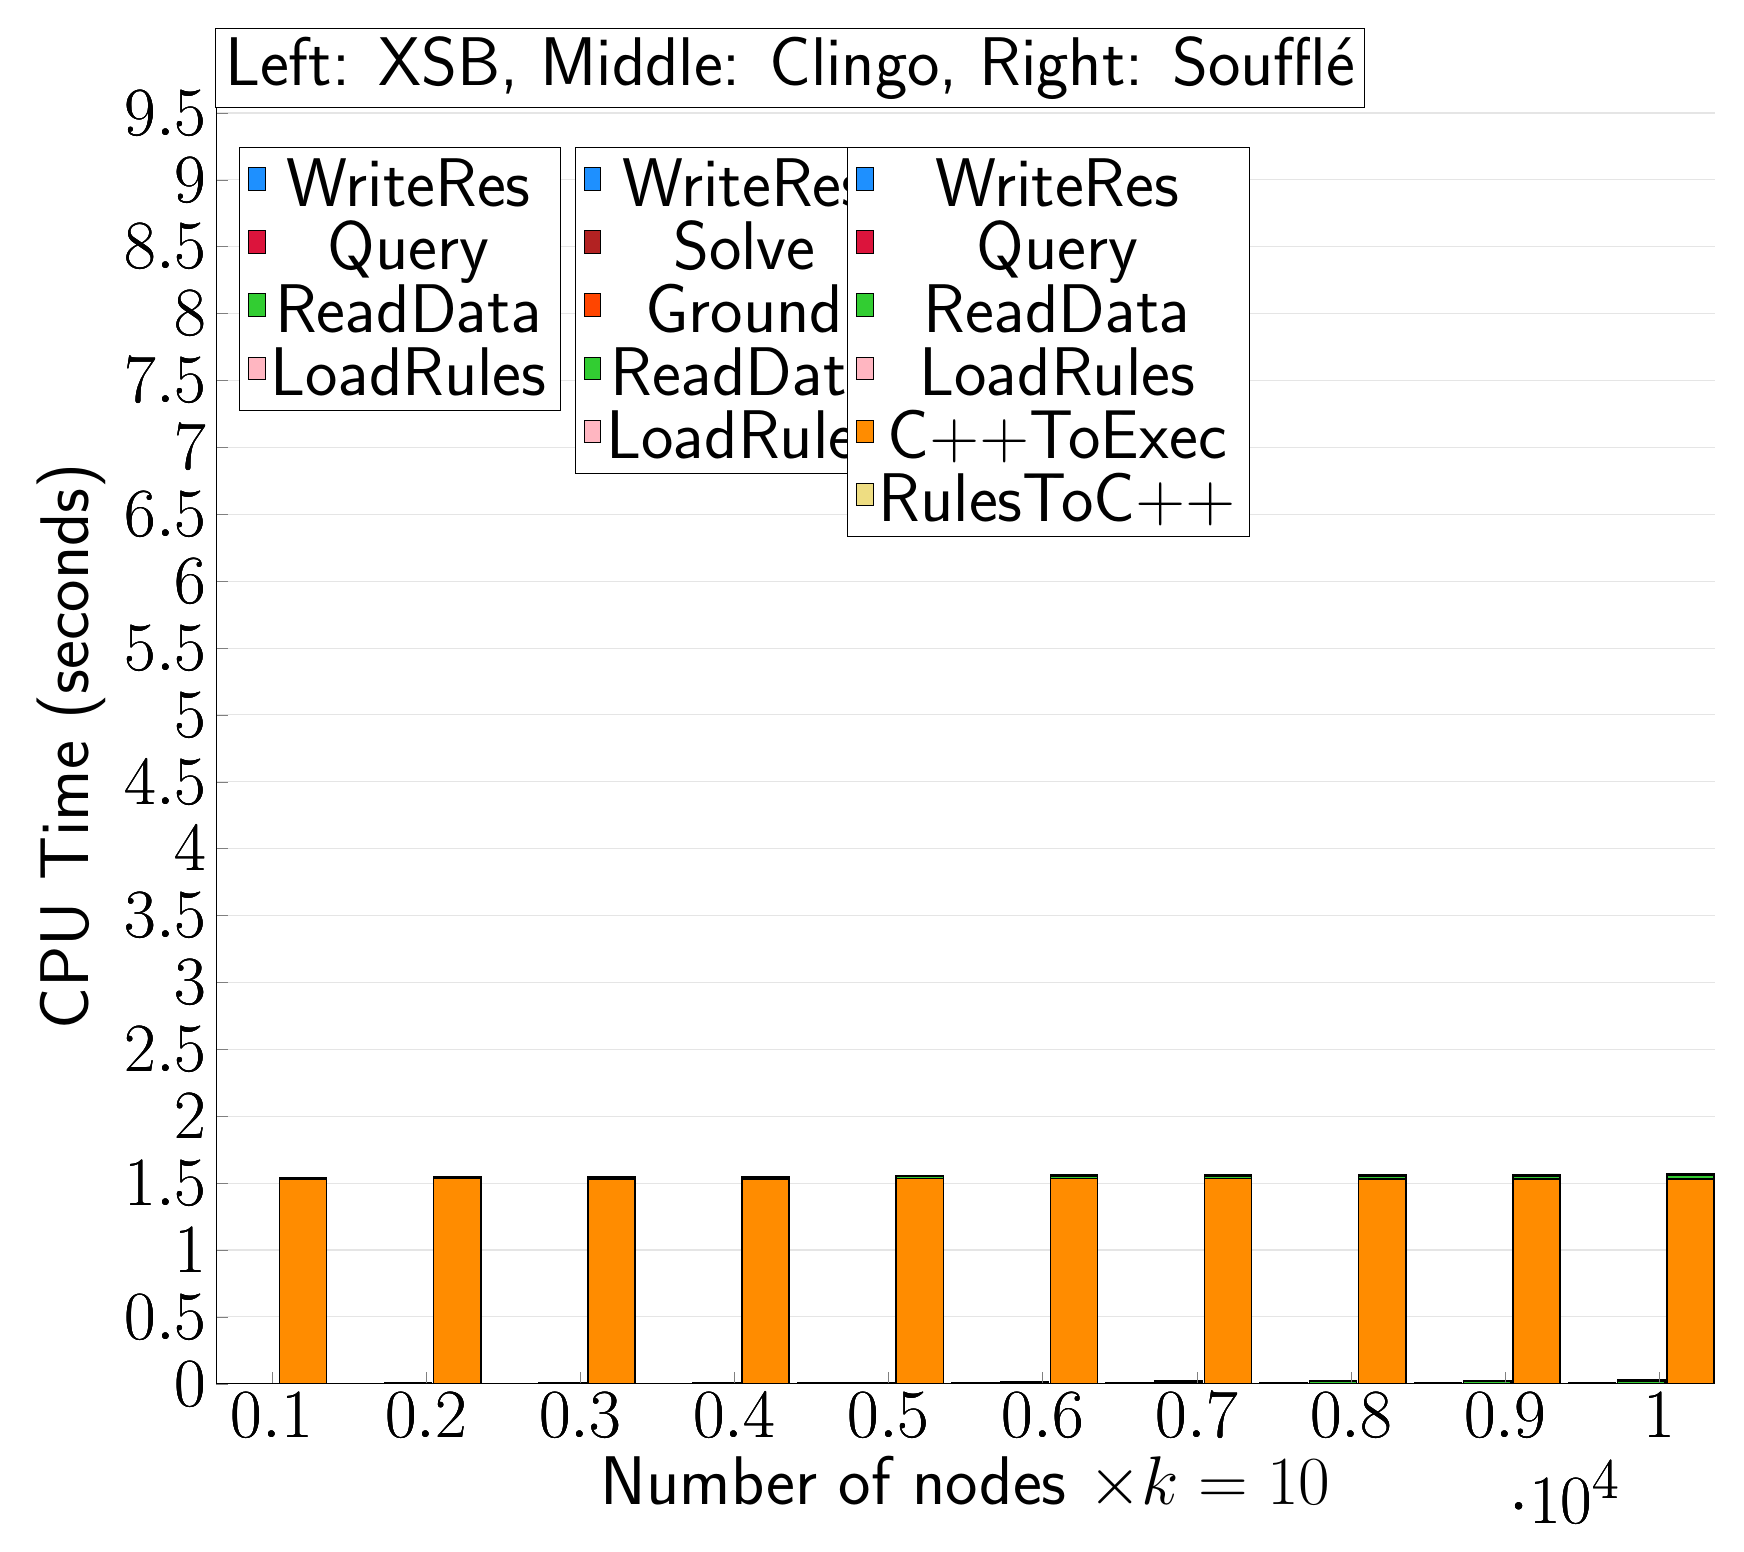
\begin{tikzpicture}
                        \begin{axis}[bar shift=-24.3pt, 
   ybar stacked,
   width=1.7\textwidth,
   bar width=0.6cm,
   ymajorgrids, tick align=inside,
   major grid style={draw=gray!20},
   xtick=data,
   ymin=0, ymax=9.534,
   axis x line*=bottom,
   axis y line*=left,
   enlarge x limits=0.04,
   legend style={
       at={(0.23, 0.97)},
       anchor=north east,
       legend columns=1,
       font=\Huge,
   },
   ylabel={CPU Time (seconds)},
   xlabel={Number of nodes $\times k=10$},
   label style={font=\Huge},
   tick label style={font=\Huge},
]
\addlegendimage{fill=DodgerBlue, draw=black, line width=0.2pt}
\addlegendentry{WriteRes}
\addlegendimage{fill=Crimson, draw=black, line width=0.2pt}
\addlegendentry{Query}
\addlegendimage{fill=LimeGreen, draw=black, line width=0.2pt}
\addlegendentry{ReadData}
\addlegendimage{fill=LightPink, draw=black, line width=0.2pt}
\addlegendentry{LoadRules}
\addplot +[fill=LightPink, draw=black, line width=0.55pt] coordinates {
(1000, 0.0005496000000000001)
(2000, 0.0005488)
(3000, 0.0005572000000000002)
(4000, 0.0005573999999999998)
(5000, 0.0005503999999999996)
(6000, 0.0005521999999999994)
(7000, 0.0005518000000000002)
(8000, 0.0005577999999999996)
(9000, 0.0005523999999999991)
(10000, 0.0005547999999999991)
};
\addplot +[fill=LimeGreen, draw=black, line width=0.55pt] coordinates {
(1000, 0.0008903999999999995)
(2000, 0.0016990000000000002)
(3000, 0.0024590000000000002)
(4000, 0.0032706)
(5000, 0.0040628)
(6000, 0.0049272000000000005)
(7000, 0.005773)
(8000, 0.0065708)
(9000, 0.0073838)
(10000, 0.0081688)
};
\addplot +[fill=Crimson, draw=black, line width=0.55pt] coordinates {
(1000, 9.400000000000034e-06)
(2000, 9.199999999999487e-06)
(3000, 9.599999999999884e-06)
(4000, 1.0399999999999994e-05)
(5000, 1.0799999999998997e-05)
(6000, 1.0800000000000398e-05)
(7000, 9.80000000000078e-06)
(8000, 1.18000000000014e-05)
(9000, 1.1599999999998402e-05)
(10000, 1.1400000000000999e-05)
};
\addplot +[fill=DodgerBlue, draw=black, line width=0.55pt] coordinates {
(1000, 6.39999999999998e-05)
(2000, 6.520000000000031e-05)
(3000, 6.659999999999999e-05)
(4000, 6.379999999999995e-05)
(5000, 6.320000000000041e-05)
(6000, 6.419999999999932e-05)
(7000, 6.399999999999909e-05)
(8000, 6.519999999999894e-05)
(9000, 6.500000000000117e-05)
(10000, 6.379999999999856e-05)
};
\end{axis}

\begin{axis}[bar shift=-6.5pt, 
   ybar stacked,
   width=1.7\textwidth,
   bar width=0.6cm,
   ymajorgrids, tick align=inside,
   major grid style={draw=none},
   xtick=data,
   ymin=0, ymax=9.534,
   axis x line*=none,
   axis y line*=none,
   enlarge x limits=0.04,
   legend style={
       at={(0.454, 0.97)},
       anchor=north east,
       legend columns=1,
       font=\Huge,
   },
   label style={font=\Huge},
   tick label style={font=\Huge},
]
\addlegendimage{fill=DodgerBlue, draw=black, line width=0.2pt}
\addlegendentry{WriteRes}
\addlegendimage{fill=FireBrick, draw=black, line width=0.2pt}
\addlegendentry{Solve}
\addlegendimage{fill=OrangeRed, draw=black, line width=0.2pt}
\addlegendentry{Ground}
\addlegendimage{fill=LimeGreen, draw=black, line width=0.2pt}
\addlegendentry{ReadData}
\addlegendimage{fill=LightPink, draw=black, line width=0.2pt}
\addlegendentry{LoadRules}
\addplot +[fill=LightPink, draw=black, line width=0.55pt] coordinates {
(1000, 0.0)
(2000, 0.0)
(3000, 0.0)
(4000, 0.0)
(5000, 0.0)
(6000, 0.0)
(7000, 0.0)
(8000, 0.0)
(9000, 0.0)
(10000, 0.0)
};
\addplot +[fill=LimeGreen, draw=black, line width=0.55pt] coordinates {
(1000, 0.0)
(2000, 0.0040000000000000036)
(3000, 0.010000000000000009)
(4000, 0.010000000000000009)
(5000, 0.010000000000000009)
(6000, 0.010000000000000009)
(7000, 0.01200000000000001)
(8000, 0.020000000000000018)
(9000, 0.020000000000000018)
(10000, 0.020000000000000018)
};
\addplot +[fill=OrangeRed, draw=black, line width=0.55pt] coordinates {
(1000, 0.0)
(2000, 0.0020000000000000018)
(3000, 0.0)
(4000, 0.0)
(5000, 0.0)
(6000, 0.008000000000000007)
(7000, 0.008000000000000007)
(8000, 0.0)
(9000, 0.0020000000000000018)
(10000, 0.006000000000000005)
};
\addplot +[fill=FireBrick, draw=black, line width=0.55pt] coordinates {
(1000, 0.0)
(2000, 0.0)
(3000, 0.0)
(4000, 0.0)
(5000, 0.0)
(6000, 0.0)
(7000, 0.0)
(8000, 0.0)
(9000, 0.0)
(10000, 0.0040000000000000036)
};
\addplot +[fill=DodgerBlue, draw=black, line width=0.55pt] coordinates {
(1000, 0.0)
(2000, 0.0)
(3000, 0.0)
(4000, 0.0)
(5000, 0.0)
(6000, 0.0)
(7000, 0.0)
(8000, 0.0)
(9000, 0.0)
(10000, -0.0040000000000000036)
};
\end{axis}

\begin{axis}[bar shift=11.3pt, 
   ybar stacked,
   width=1.7\textwidth,
   bar width=0.6cm,
   ymajorgrids, tick align=inside,
   major grid style={draw=none},
   xtick=data,
   ymin=0, ymax=9.534,
   axis x line*=none,
   axis y line*=none,
   enlarge x limits=0.04,
   legend style={
       at={(0.69, 0.97)},
       anchor=north east,
       legend columns=1,
       font=\Huge,
   },
   label style={font=\Huge},
   tick label style={font=\Huge},
]
\addlegendimage{fill=DodgerBlue, draw=black, line width=0.2pt}
\addlegendentry{WriteRes}
\addlegendimage{fill=Crimson, draw=black, line width=0.2pt}
\addlegendentry{Query}
\addlegendimage{fill=LimeGreen, draw=black, line width=0.2pt}
\addlegendentry{ReadData}
\addlegendimage{fill=LightPink, draw=black, line width=0.2pt}
\addlegendentry{LoadRules}
\addlegendimage{fill=DarkOrange, draw=black, line width=0.2pt}
\addlegendentry{C++ToExec}
\addlegendimage{fill=LightGoldenrod, draw=black, line width=0.2pt}
\addlegendentry{RulesToC++}
\addplot +[fill=LightGoldenrod, draw=black, line width=0.55pt] coordinates {
(1000, 0.0)
(2000, 0.0)
(3000, 0.0)
(4000, 0.0)
(5000, 0.0)
(6000, 0.0)
(7000, 0.0020000000000000005)
(8000, 0.0020000000000000005)
(9000, 0.0)
(10000, 0.0020000000000000005)
};
\addplot +[fill=DarkOrange, draw=black, line width=0.55pt] coordinates {
(1000, 1.532)
(2000, 1.5400000000000003)
(3000, 1.53)
(4000, 1.528)
(5000, 1.5340000000000003)
(6000, 1.536)
(7000, 1.5340000000000003)
(8000, 1.53)
(9000, 1.5299999999999998)
(10000, 1.53)
};
\addplot +[fill=LightPink, draw=black, line width=0.55pt] coordinates {
(1000, 0.00015179999999999998)
(2000, 0.0001422)
(3000, 0.0001466)
(4000, 0.00014580000000000002)
(5000, 0.00015279999999999997)
(6000, 0.0001472)
(7000, 0.0001438)
(8000, 0.0001378)
(9000, 0.0001524)
(10000, 0.000152)
};
\addplot +[fill=LimeGreen, draw=black, line width=0.55pt] coordinates {
(1000, 0.003772)
(2000, 0.007011399999999999)
(3000, 0.0095768)
(4000, 0.0117462)
(5000, 0.0143316)
(6000, 0.0165114)
(7000, 0.0187586)
(8000, 0.020879599999999998)
(9000, 0.0232252)
(10000, 0.0245072)
};
\addplot +[fill=Crimson, draw=black, line width=0.55pt] coordinates {
(1000, 0.0016175999999999999)
(2000, 0.0028646)
(3000, 0.004315)
(4000, 0.0055292)
(5000, 0.006396000000000001)
(6000, 0.0070326)
(7000, 0.008374000000000001)
(8000, 0.008963599999999999)
(9000, 0.009076399999999998)
(10000, 0.0103186)
};
\addplot +[fill=DodgerBlue, draw=black, line width=0.55pt] coordinates {
(1000, 0.0003468)
(2000, 0.00026419999999999997)
(3000, 0.00028340000000000006)
(4000, 0.0002728)
(5000, 0.0002622)
(6000, 0.00025279999999999996)
(7000, 0.0002652)
(8000, 0.00024080000000000005)
(9000, 0.0002366)
(10000, 0.00027)
};
\end{axis}


\node[anchor=south, draw, fill=white] at (rel axis cs:0.42,1) {\Huge Left: XSB, Middle: Clingo, Right: Soufflé};
\end{tikzpicture}
\end{document}
                    